\label{appendix:presion}

Este apéndice está destinado a aclarar el significado de la "presión social" actuando sobre un individuo y la presión colectiva (presión de \textit{bulk}).  
\\
\section{\label{social_pressure}La presión social}

La figura ~\ref{hilera2} representa una hilera de individuos empujando a la derecha. La pared impide el movimiento de los peatones. Todos los individuos de la hilera están en su posición de equilibrio $x_1,x_2,...,x_{i},...x_N$, mientras que la pared está en la posición $x_0=0$. 

\begin{figure}[!htbp]
\center
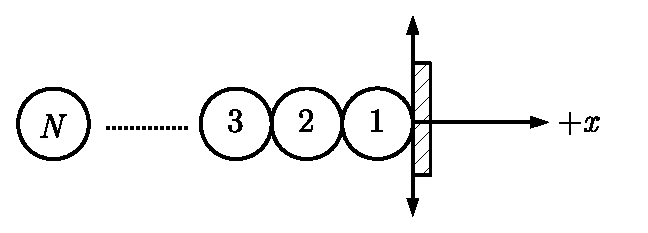
\includegraphics[scale=1]{figuras/hilera.eps}
\caption{\label{hilera2} Hilera de individuos empujando a la derecha. El eje horizontal indica la posición positiva. }
% done with figuras_presion.odg
\end{figure}

Los peatones empujan a la derecha gracias a la fuerza de deseo
$f_d^{(i)}=mv_d/\tau$, según la Ec.~(\ref{fdeseo}). La repulsión social balancea la fuerza de deseo, pero solo se tiene en cuenta la interacción de los individuos en contacto (se desprecia la interacción de segundos vecinos). La Ec ~\ref{eqn_6} muestra la ecuación de balance de cada individuo en la hilera. \\

\begin{equation}
 f_s^{(i,i+1)}-f_s^{(i,i-1)}+\displaystyle\frac{mv_d}{\tau}=0\label{eqn_6}
\end{equation}

\noindent con $f_s^{(i,j)}$ la fuerza repulsiva que siente el individuo $i$ debido a la presencia del peatón $j$. Cabe destacar que la condición de contorno en la posición $x_0=0$  es condición de Dirichlet, mientras que la condición en el otro extremos es condición de Neumann $f_s^{(N,N+1)}=0$. Las fuerzas en los peatones se obtienen de forma recursiva a partir de la expresión~\ref{eqn_6}, empezando desde el extremo libre ($i=N$). El resultado es

\begin{equation}
f_s^{(i,i-1)}=(N-i+1)\,\displaystyle\frac{mv_d}{\tau}\ \ \ , \ \ \ 
i=1,....,N\label{eqn_7}
\end{equation}

\noindent con las correspondientes posiciones  $x_1,x_2,...,x_{i},...x_N$ obtenidas a partir de la sustitución de la fuerza social expresada en Ec.~\ref{fsocial}, comenzando en la posición de la pared.

\begin{equation} 
x_i=x_{i-1}-(r_{i}+r_{i-1})+B\,\ln\bigg[(N-i+1)\,\displaystyle\frac{mv_d}{A\tau}
\bigg]\label{eqn_8}
\end{equation}

La intuición sugiere que la presión que siente un peatón $P_i$ 
corresponde a las fuerzas actuando en él (por unidad de área) debido a los primeros vecinos. De la definición de "función de presión social" (\ref{pa}) se puede derivar

\begin{equation}
P_i=\displaystyle\frac{1}{2}\,\bigg[\displaystyle\frac{x_{i}-x_{i+1}}{2VA_i}\,
f_s^ { (i , i+1) } +\displaystyle\frac { x_ {i-1}-x_{i}}{2A_i}\,f_s^{(i,i-1) 
}\bigg]\label{eqn_9}
\end{equation}

\vspace{3mm}

\noindent donde la magnitud $x_{ij}/2A_i$ corresponde a la inversa de la superficie efectiva del peatón. Para individuos modelados como esferas rígidas, la distancia entre peatones es $x_{ij}=2r_i$ y el área $A_i=4\pi r_i^3/3$. Por lo tanto, 

\begin{equation}
P_i=\displaystyle\frac{1}{4\pi 
r_i^2}\,\bigg[f_s^ { (i , i+1) } +f_s^{(i,i-1)}\bigg]\label{eqn_10}
\end{equation}

\noindent como es de esperar para la presión del individuo.  \\

\section{\label{bulk_pressure}La presión de bulk}

Se puede verificar la relación de virial (\ref{virial2}) a través de la expresión (\ref{eqn_9}). Agregando los términos de la hilera de $N$ peatones y reemplazando el primer y último término por las correspondientes condiciones de contorno. Esto da como resultado,


\begin{equation}
\left\{\begin{array}{lcl}
2P_1A_1 
& = &\displaystyle\frac{x_{1}}{2}f_s^ { (1 , 2)} - 
\displaystyle\frac{x_{2}}{2}\,f_s^ { (1 , 2) }  \\
&& \\
2P_2A_2 
& = &\displaystyle\frac{x_{2}}{2}\,\big[f_s^ { (2 , 3)} - f_s^{(2,1)} 
\big] - \displaystyle\frac{x_{3}}{2}\,f_s^ { (2 , 3) } +\displaystyle\frac 
{ x_ {1}}{2}\,f_s^{(2,1) 
} \\
&& \\
2P_3A_3 
& = &\displaystyle\frac{x_{3}}{2}\,\big[f_s^ { (3 , 4)} - f_s^{(3,2)} 
\big] - \displaystyle\frac{x_{4}}{2}\,f_s^ { (3 , 4) } +\displaystyle\frac 
{ x_{2}}{2}\,f_s^{(3,2) 
} \\
... &&\\
&& \\
2P_NA_N 
& = &-\displaystyle\frac{x_{N}}{2}\, f_s^{(N,N-1)} 
+\displaystyle\frac{ x_{N-1}}{2}\,f_s^{(N,N-1) 
} \\
 \end{array}\right.\label{eqn_11}
\end{equation}

Estas son las presiones locales en cada peatón debido al contacto entre individuos (excluyendo las paredes). La suma de los términos resulta la ecuación de virial como esta expresada en (\ref{virial2})

\begin{equation}
\begin{array}{lcl}
\displaystyle\sum_{i=1}^N 2P_iA_i & = & (x_1 - x_2)f_s^{(1,2)} + (x_2 - 
x_3)f_s^{(2,3)} +... \\
& + &  (x_{N-1}-x_N)f_s^{(N,N-1)} \\
&& \\
& = & x_{1}\,\displaystyle\frac{N\,mv_d}{\tau} - 
\displaystyle\sum_{i=1}^N x_i\,\displaystyle\frac{mv_d}{\tau} \\
 \end{array}\label{eqn_12}
\end{equation}

\noindent donde el primer término corresponde a la presión global
$-2\mathcal{PA}$. Notar que $x_1$ es negativo, y $2\mathcal{PA}$ es definido positivo. El último término también es positivo, le agrega presión al bulk debido a las fuerzas de deseo.  
\\
La relación de virial (\ref{virial2}) permite calcular la presión de \textit{bulk} en un grupo de peatones. Por ejemplo, la presión en los  $M$ peatones más cercanos a la pared corresponde a la fuerza actuando en este grupo debido a los $N-M$ restantes. Según la Ec.~(\ref{virial2}), la presión en los $M$ individuos es


\begin{equation}
 \displaystyle\sum_{i=1}^M 2P_iA_i 
=-2\mathcal{PA}-\displaystyle\sum_{i=M+1}^N 2P_iA_i-\displaystyle\sum_{i=1}^N 
x_i\displaystyle\frac{mv_d}{\tau}\label{eqn_13}
\end{equation}

La presión de bulk en los primeros $M$ individuos aumenta con la cantidad de peatones incluidos en la multitud. Esto se verifica evaluando las ecuaciones~(\ref{eqn_12}) y (\ref{eqn_13}) incrementando el valor de $N$.\\

Las Ecs~(\ref{eqn_7}) y (\ref{eqn_8}) permiten calcular el perfil de presiones en función de la distancia a la pared. El perfil es similar al medido en un proceso de evacuación.

La figura~\ref{fis_g} representa una curva de la presión en cada peatón. \\

\begin{figure}[H]
    \centering
    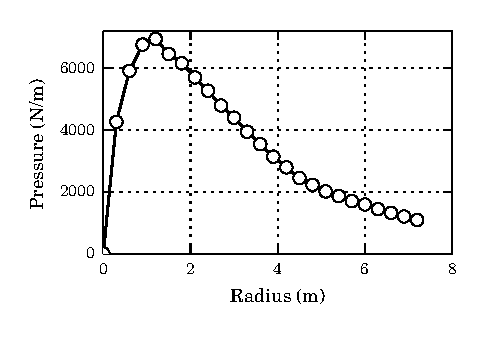
\includegraphics[scale=1]{figuras/p_dist.eps}
    \caption[width=5cm]{Presión media en función de la distancia a la salida. El tamaño del recinto fue $20\,\mathrm{m}\times20\,\mathrm{m}$  con una puerta de $L=1.2$~m width. Los valores medios fueron calculados a partir de 30 procesos hasta que 100 peatones abandonaron la habitación. La velocidad de deseo fue $v_d=4\,$m/s. La distancia a la puerta fue dividida en bins de tamaño $0.3$~m o 1~m.  El símbolo $\bigcirc$  corresponde a bins de $0.3$~m.}
    \label{fis_g}
\end{figure}



